\documentclass[UTF8]{article}
\usepackage{ctex}
\usepackage{geometry}
\usepackage{float}
\usepackage{graphicx}
\usepackage{listings}
\usepackage{subfigure}
\usepackage{amsmath}
\usepackage{textcomp}
\usepackage{booktabs}
\geometry{a4paper,left=2cm,right=2cm,top=2cm,bottom=2cm}
\title{热电偶分度校验实验}
\author{能动A71 宋德培 2174110112}

\renewcommand{\thesection}{\Roman{section}}
\renewcommand{\thesubsection}{\arabic{section} .\arabic{subsection}}
\usepackage{xcolor}
\lstset{
	numbers=left, 
	numberstyle= \tiny, 
	keywordstyle= \color{ blue!70},
	commentstyle= \color{red!50!green!50!blue!50}, 
	frame=shadowbox, % 阴影效果
	rulesepcolor= \color{ red!20!green!20!blue!20} ,
	escapeinside=``, % 英文分号中可写入中文
	xleftmargin=2em,xrightmargin=2em, aboveskip=1em,
	framexleftmargin=2em
} 

\makeatletter
\newcommand{\rmnum}[1]{\romannumeral #1}
\newcommand{\Rmnum}[1]{\expandafter\@slowromancap\romannumeral #1@}
\makeatother

\begin{document}
	\maketitle
	\section{实验目的}
	1.	观察热电偶的结构,获得有关感性知识;
	
	2.	理解热电偶校验系统的工作原理,掌握热电偶的使用方法;
	
	3.	熟悉相关仪器设备的基本特性和使用方法。
	
	\section{实验原理}
	本实验使用比较法进行热电偶的校验,检验温度根据热电偶型号选择为$400$\textcelsius、600\textcelsius、800\textcelsius。采用事先校验过的镍铬——镍硅电偶作为标准热电偶。
	
	将标准热电偶和被校验热电偶置于检定炉中,参考端置于半导体零度恒温器中,使用同一个电位差计连接两个热电偶,并在校验点上交替读取标准热电偶和被校验热电偶的电势差,然后对读数取平均值。
	
	\section{操作步骤要点}
	1. 观察温控设备测量值显示窗口(PV)数值变化情况,待其稳定在校验点±10 ℃的范围之内 (炉温变化不得超过 0.2℃/分) 时,方可读数。
	
	2. 两个热电偶的电势交替读取,标准热电偶5次,被校热电偶4次。
	\section{数据处理}
	\subsection{数据处理示例}
	以$400$\textcelsius 校验点为例,标准热电偶电势测量平均值为$E(400,0) = 16.345\ $mV,检定结果为$E_s = 16.414\ $mV,K(EU-2)热电偶分度表中对应电势值$E_t = 16.397\ $mV,因此可以计算出
	\[
	\Delta E = E_t-E_s = -0.017 \ \mathrm{mV}
	\]
	因此
	\[
	E = E(t,0) +\Delta E = 16.328\ \mathrm{mV}
	\]
	通过查电偶分度表,可以获得实际炉内温度$t = 398.4$\textcelsius,而$E^{'}(400,0) = 16.367\ $mV,通过热电偶分度表查得温度$t^{'} = 399.3$\textcelsius,因此
	\[
	\Delta t = t^{'} - t = 0.9 ^\circ \mathrm{C}
	\]
	由于在$400$\textcelsius 时,在\Rmnum{2}级精度下允许误差为$\pm 3$\textcelsius,因此误差在允许范围内。
	
	下面给出所有校验点的结果
	\begin{table}[H]
		\centering
		\caption{检验点检验结果}
	\begin{tabular}{cccc}
		\toprule
		校验点&误差/$^\circ$C  & 允许误差/$\pm ^\circ$C & 是否合格 \\ 
		\midrule
		$400^\circ$C&0.9  &3  &是  \\ 
		$600^\circ$C& 1.6 &4.5  &是  \\ 
		$800^\circ$C&  2.2& 6.0 & 是 \\ 
		\bottomrule
	\end{tabular}
	\end{table}

\subsection{检定结果}
	因此,在所有校验点上被测热电偶通过校验,可以认为该热电偶在\Rmnum2 级精度下合格。
	
	\section{附录——原始数据记录}
	\begin{figure}[H]
		\centering
		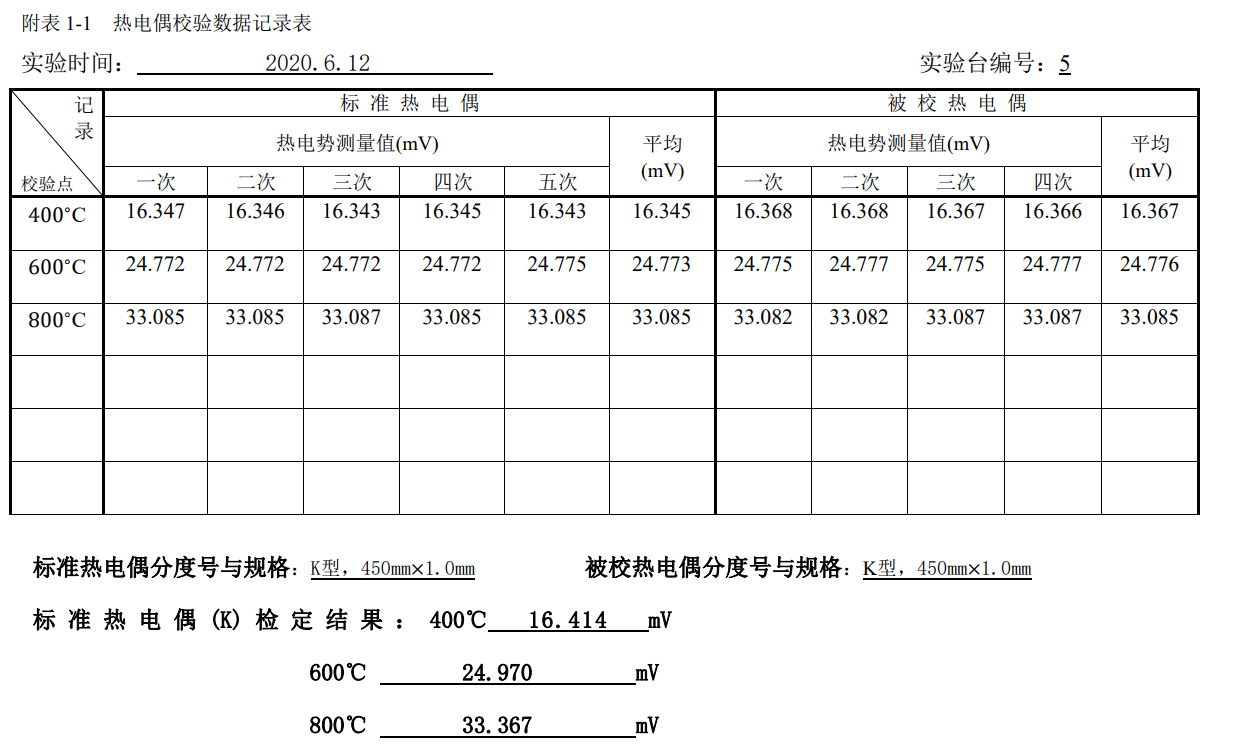
\includegraphics[width=\linewidth]{figure/origin}
		\label{fig:origin}
	\end{figure}
	
\end{document}